\documentclass{article}
\usepackage{fullpage}
\usepackage{amsmath}
\usepackage{amsfonts}
\usepackage{tipa}
\usepackage{tikz}
\newcommand\myeq{\mathrel{\stackrel{\makebox[0pt]{\mbox{\normalfont\tiny def}}}{=}}}
\begin{document}
\begin{center}
\Large{Tone Sandhi in Shanghai Wu}
\end{center} 
\vspace{.5cm} 
\par \indent
Here, I will attempt to offer logical characterizations of tone sandhi patterns in two dialects of Chinese: Shanghai (Wu) and Tianjin (Mandarin).\\
\indent
For the Shanghai data, I would like to focus on more recent phonetic evidence from Chen (2008) that simplifies characterizations of tone sandhi. Her results suggest a mapping in which all non-initial (initial $\sigma$) tone-to-TBU associations delete, associating instead to a [L] target throughout the rest of the domain, crucially even as early as the first non-initial syllable.
\vspace{.3cm}
\begin{center}
\begin{tabular} {rlllll}
	& $\sigma 1$ & $\sigma 2$ & $\sigma 3$ & $\sigma 4$ & $\sigma 5$ \\
	\hline
	underlying form & HL & LH& LH & MH & HL \\
	sandhi form & HL & \textbf{L} & \textbf{L} & \textbf{L} & \textbf{L} \\
	\hline
\end{tabular}\\
\smallskip{}
Table 1: Shanghai tone sandhi over a pentasyllabic domain
\end{center}	
\vspace{.3cm}
Therefore, regardless of the specification of the lexical tone, non-initial syllables always default to [L]. The domain-initial syllable retains its underlying melodic realization, but the melody does not spread over the entire domain as previously thought.\\
\indent
Adopting the autosegmental representational formalism employed by Jardine (2016) to characterize tonal mappings in Zigula and Shambaa, there are a variety of alternatives available for representing Shanghai tone sandhi. A crucial choice to consider concerns underlying specifications of associations between tones and TBUs. Figure 1 assumes no underlying specification.
\begin{center}
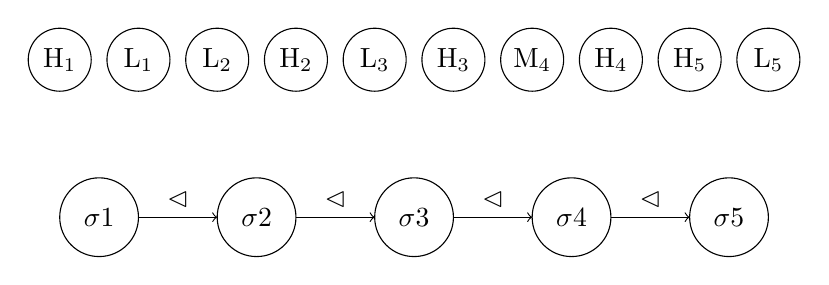
\begin{tikzpicture}
	\draw (-5.5,2) circle [radius = .4] node {H$_1$};
	\draw (-4.5,2) circle [radius = .4] node {L$_1$};
	\draw (-5, 0) circle [radius = .5] node {$\sigma1$};
	\draw (-3.5,2) circle [radius = .4] node {L$_2$};
	\draw (-2.5,2) circle [radius = .4] node {H$_2$};
	\draw (-3, 0) circle [radius = .5] node {$\sigma2$};
	\draw (-1, 0) circle [radius = .5] node {$\sigma3$};
	\draw (-1.5,2) circle [radius = .4] node {L$_3$};
	\draw (-.5,2) circle [radius = .4] node {H$_3$};
	\draw (1, 0) circle [radius = .5] node {$\sigma4$};
	\draw (.5,2) circle [radius = .4] node {M$_4$};
	\draw (1.5,2) circle [radius = .4] node {H$_4$};
	\draw (2.5,2) circle [radius = .4] node {H$_5$};
	\draw (3.5,2) circle [radius = .4] node {L$_5$};
	\draw (3, 0) circle [radius = .5] node {$\sigma5$};
	\draw [->] (-4.5,0) -- (-3.5,0) node [above, pos=.5] {$\lhd$};
	\draw [->] (-2.5,0) -- (-1.5,0) node [above, pos=.5] {$\lhd$};
	\draw [->] (-.5,0) -- (.5,0) node [above, pos=.5] {$\lhd$};
	\draw [->] (1.5,0) -- (2.5,0) node [above, pos=.5] {$\lhd$};
	
\end{tikzpicture}
\end{center}
\vspace{.3cm}
\begin{center}
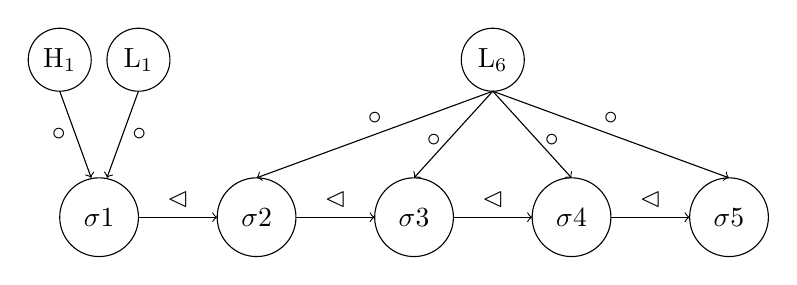
\begin{tikzpicture}
	\draw (-5.5,2) circle [radius = .4] node {H$_1$};
	\draw (-4.5,2) circle [radius = .4] node {L$_1$};
	\draw (0, 2) circle [radius = .4] node {L$_6$};
	\draw (-5, 0) circle [radius = .5] node {$\sigma1$};
	\draw (-3, 0) circle [radius = .5] node {$\sigma2$};
	\draw (-1, 0) circle [radius = .5] node {$\sigma3$};
	\draw (1, 0) circle [radius = .5] node {$\sigma4$};
	\draw (3, 0) circle [radius = .5] node {$\sigma5$};
	\draw [->] (-4.5,0) -- (-3.5,0) node [above, pos=.5] {$\lhd$};
	\draw [->] (-2.5,0) -- (-1.5,0) node [above, pos=.5] {$\lhd$};
	\draw [->] (-.5,0) -- (.5,0) node [above, pos=.5] {$\lhd$};
	\draw [->] (1.5,0) -- (2.5,0) node [above, pos=.5] {$\lhd$};
	\draw [->] (-5.5,1.6) -- (-5.1,.5) node [left, pos = .5] {$\circ$};
	\draw [->] (-4.5,1.6) -- (-4.9,.5) node [right, pos = .5] {$\circ$};
	\draw [->] (0, 1.6) -- (-3, .5) node [above, pos = .5] {$\circ$};
	\draw [->] (0, 1.6) -- (-1, .5) node [above, pos = .75] {$\circ$};
	\draw [->] (0, 1.6) -- (1, .5) node [above, pos = .75] {$\circ$};
	\draw [->] (0, 1.6) -- (3, .5) node [above, pos = .5] {$\circ$};
	
\end{tikzpicture}\\
\smallskip{}
Figure 1: Autosegmental representation for Shanghai tone sandhi (no associations)
\end{center}
There are good reasons, however, to posit underlying associations. Dealing solely with a system in which [H] and [L] are tonal primitives (that is, excluding [R] rising and [F] falling contours from our set of melodic atoms), it is difficult to formalize a grammar that would associate both [H] and [L] in domains whose initial syllables have contour tones but associate only one of [H] or [L] in words whose domain-initial syllables are a high or low level tone. Without associations specified underlyingly, the choice between the two is arbitrary.\\
\indent
Therefore, we will posit a model in which each syllable is specified for tone, and associations are present underlyingly, as in Figure 2.
\begin{center}
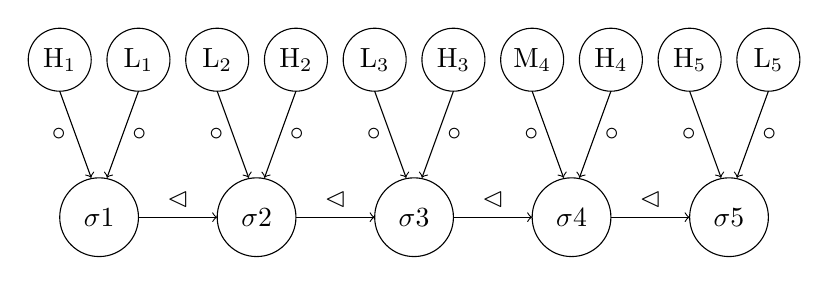
\begin{tikzpicture}
	\draw (-5.5,2) circle [radius = .4] node {H$_1$};
	\draw (-4.5,2) circle [radius = .4] node {L$_1$};
	\draw (-5, 0) circle [radius = .5] node {$\sigma1$};
	\draw (-3.5,2) circle [radius = .4] node {L$_2$};
	\draw (-2.5,2) circle [radius = .4] node {H$_2$};
	\draw (-3, 0) circle [radius = .5] node {$\sigma2$};
	\draw (-1, 0) circle [radius = .5] node {$\sigma3$};
	\draw (-1.5,2) circle [radius = .4] node {L$_3$};
	\draw (-.5,2) circle [radius = .4] node {H$_3$};
	\draw (1, 0) circle [radius = .5] node {$\sigma4$};
	\draw (.5,2) circle [radius = .4] node {M$_4$};
	\draw (1.5,2) circle [radius = .4] node {H$_4$};
	\draw (2.5,2) circle [radius = .4] node {H$_5$};
	\draw (3.5,2) circle [radius = .4] node {L$_5$};
	\draw (3, 0) circle [radius = .5] node {$\sigma5$};
	\draw [->] (-4.5,0) -- (-3.5,0) node [above, pos=.5] {$\lhd$};
	\draw [->] (-2.5,0) -- (-1.5,0) node [above, pos=.5] {$\lhd$};
	\draw [->] (-.5,0) -- (.5,0) node [above, pos=.5] {$\lhd$};
	\draw [->] (1.5,0) -- (2.5,0) node [above, pos=.5] {$\lhd$};
	\draw [->] (-5.5,1.6) -- (-5.1,.5) node [left, pos = .5] {$\circ$};
	\draw [->] (-4.5,1.6) -- (-4.9,.5) node [right, pos = .5] {$\circ$};
	\draw [->] (-3.5,1.6) -- (-3.1,.5) node [left, pos = .5] {$\circ$};
	\draw [->] (-2.5,1.6) -- (-2.9,.5) node [right, pos = .5] {$\circ$};
	\draw [->] (-1.5,1.6) -- (-1.1,.5) node [left, pos = .5] {$\circ$};
	\draw [->] (-0.5,1.6) -- (-0.9,.5) node [right, pos = .5] {$\circ$};
	\draw [->] (.5,1.6) -- (.9,.5) node [left, pos = .5] {$\circ$};
	\draw [->] (1.5,1.6) -- (1.1,.5) node [right, pos = .5] {$\circ$};
	\draw [->] (2.5,1.6) -- (2.9,.5) node [left, pos = .5] {$\circ$};
	\draw [->] (3.5,1.6) -- (3.1,.5) node [right, pos = .5] {$\circ$};
	
\end{tikzpicture}
\end{center}
\vspace{.3cm}
\begin{center}
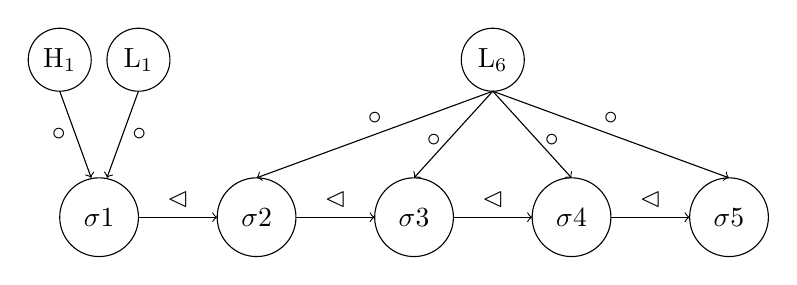
\begin{tikzpicture}
	\draw (-5.5,2) circle [radius = .4] node {H$_1$};
	\draw (-4.5,2) circle [radius = .4] node {L$_1$};
	\draw (0, 2) circle [radius = .4] node {L$_6$};
	\draw (-5, 0) circle [radius = .5] node {$\sigma1$};
	\draw (-3, 0) circle [radius = .5] node {$\sigma2$};
	\draw (-1, 0) circle [radius = .5] node {$\sigma3$};
	\draw (1, 0) circle [radius = .5] node {$\sigma4$};
	\draw (3, 0) circle [radius = .5] node {$\sigma5$};
	\draw [->] (-4.5,0) -- (-3.5,0) node [above, pos=.5] {$\lhd$};
	\draw [->] (-2.5,0) -- (-1.5,0) node [above, pos=.5] {$\lhd$};
	\draw [->] (-.5,0) -- (.5,0) node [above, pos=.5] {$\lhd$};
	\draw [->] (1.5,0) -- (2.5,0) node [above, pos=.5] {$\lhd$};
	\draw [->] (-5.5,1.6) -- (-5.1,.5) node [left, pos = .5] {$\circ$};
	\draw [->] (-4.5,1.6) -- (-4.9,.5) node [right, pos = .5] {$\circ$};
	\draw [->] (0, 1.6) -- (-3, .5) node [above, pos = .5] {$\circ$};
	\draw [->] (0, 1.6) -- (-1, .5) node [above, pos = .75] {$\circ$};
	\draw [->] (0, 1.6) -- (1, .5) node [above, pos = .75] {$\circ$};
	\draw [->] (0, 1.6) -- (3, .5) node [above, pos = .5] {$\circ$};
	
\end{tikzpicture}\\
\smallskip{}
Figure 2: Autosegmental representation for Shanghai tone sandhi (associations specified)
\end{center}
\smallskip{}
We will adopt Jardine's (2016) framework (unary relations for tone, the binary successor and association relations, tonal wellformedness conditions, etc.) but with minor alterations, namely that TBUs are just defined as syllabic elements in the model.
\begin{center} 
$\varphi _{\mathsf{TBU}} (x) \myeq \sigma (x)$
\end{center} 
We also want to define a predicate that identifies the first syllable on the syllabic tier. This will be similar to Jardine's (2016) $\varphi _{\mathsf{finalV}} (x)$:
\begin{center}
$\varphi _{\mathsf{initial}\sigma}(x) \myeq \sigma (x) \wedge (\forall y) [ (x < y)]$
\end{center}
That is, it is a syllable succeeded by every other syllable.\\
\indent
Since associations between tones and TBUs are specified underlyingly, this will require an input signature that specifies the binary association relation. There will also be an output association relation in the output signature, as shown below:
\begin{center}
\begin{tabular}{l}
$\langle D; <, P_{\sigma}, P_{H}, P_{L}, \circ \rangle$\\
$\langle D'; <_{o}, R_{\sigma}, R_{H}, R_{L}, \circ_{o} \rangle$\\
\end{tabular}
\end{center}
We can then set the copy set to {1}; the output copy will contain two tiers.\\
The next step is to define the output unary relations. These are defined in terms of the input relations:
\begin{center}
\begin{tabular}{l}
$R^{1}_{\mu}(x) \myeq P_{\mu}(x)$\\
$R^{1}_{H}(x) \myeq P_{H}(x)$\\
$R^{1}_{L}(x) \myeq P_{L}(x)$\\
\end{tabular}
\end{center}
The association relation on the first copy set is defined as below:
\begin{center}
$x \circ^{1,1}_{o} y \myeq [\mathsf{initial}_{\sigma}(x) \wedge x \circ y] \vee [(\neg  \mathsf{initial}_{\sigma}(x)) \wedge \varphi_{L}(y)]$
\end{center}
Here, output association between tones and TBUs preserves input association only on the first syllable (first conjunct); any non-initial syllable associates to a default [L] tone (second conjunct).
\pagebreak
\begin{center} References \end{center}
\smallskip{}
\hangindent=.5cm
Chen, Yiya. 2008. Revisiting the phonetics and phonology of Shanghai tone sandhi. \textit{Proceedings of the Fourth Conference on Speech Prosody}: 253-256.\\
\par \noindent
Jardine, Adam. 2016. Autosegmental representations in Zigula and Shambaa. Ms, Rutgers.
\end{document}
